\setcounter{section}{2}
\setcounter{subsection}{1}
\setcounter{answer}{0}

\subsection{Chapter 2: Creating graphs from data}

\answer{
    \vspace*{10pt}
    \begin{center}
    \begin{tabular}{|c|c|c|c|}
    \hline
    0 to 2 & 2 to 4 & 4 to 6 & 6 to 8 \tstrut\bstrut\\
    \hline
    & & & \\
    Frequency: 4  & Frequency: 5 & Frequency: 3 & Frequency: 3 \bstrut\\
    \hline
    \end{tabular}
    \end{center}
}

\answer{
\vspace*{10pt}
\begin{center}
    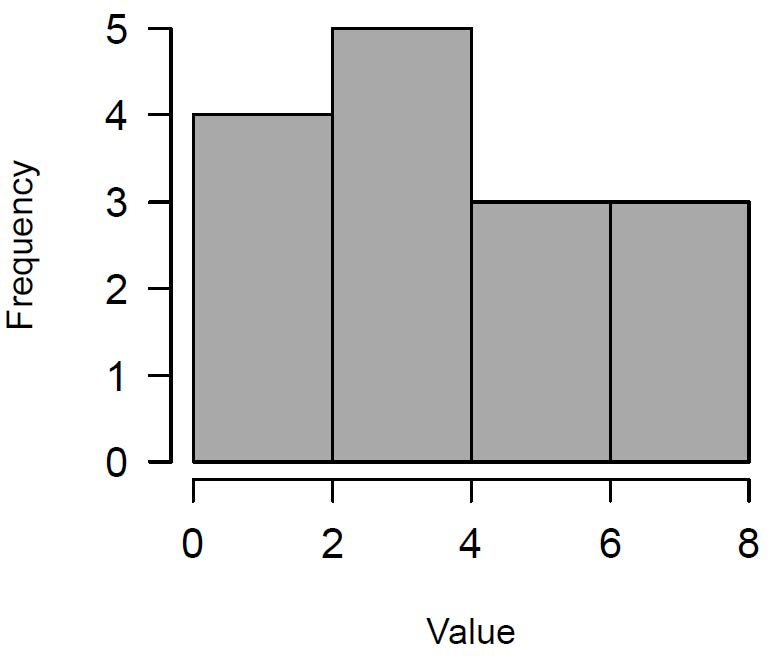
\includegraphics[width=.4\textwidth]{Files/Images/answer2.1b.jpg}
    \end{center}
}

\answerbreakline \setcounter{subsection}{2} \setcounter{answer}{0}

\answer{
    In the plot window you can see that a histogram for the values in the variable \rcode{dataset4} has been drawn by \texttt{R}. \\
    \\
    \answercode{dataset4 <- c(1.5, 5.5, 1.7, 7.2, 1.2, 7.9, 1.4, 3.6, \\
                              3.1, 3.8, 5.9, 3.6, 5.1, 3.2, 7.1) \\
                hist(dataset4)}
}

\answer{
    The histogram drawn by \texttt{R} has four bars for the ranges 1-2, 3-4, 5-6, and 7-8. The histogram from assignment 2.1b has four bars for the ranges 0-2, 2-4, 4-6, and 6-8. The difference in these two histograms is that they have a different number of bars for different ranges.
}

\answer{
    \vspace*{-10pt}
    \answercode{{\color{dataset}\# The breaks argument determines the number of bars in the histogram} \\ 
{\color{dataset}\# see ?hist for more help on the hist() function} \\ 
hist(dataset4, breaks = 4)}
}

\answer{
    \vspace*{-10pt}
    \answercode{hist(dataset4, breaks = 4, col = \textquotesingle blue\textquotesingle,  {\color{dataset}\# col sets the bar color} \\
     xlab = \textquotesingle x-axis\textquotesingle,                     {\color{dataset}\# xlab sets the x-axis name} \\
     ylab = \textquotesingle Frequency\textquotesingle,                  {\color{dataset}\# ylab sets the y-axis name} \\
     main = \textquotesingle My histogram\textquotesingle)               {\color{dataset}\# main sets the title}}
}

\clearpage % Page break

\answer{
    These data are positively skewed.  \\
    \\
\underline{Explanation}: The mean is higher than the median, and so more values are concentrated on the left side (tail) of the distribution graph while the right tail of the distribution graph is longer. \\
\\
\answercode{mean(dataset4)    {\color{dataset}\# Mean: 4.12} \\
median(dataset4)  {\color{dataset}\# Median: 3.6}}
}

\answerbreakline \setcounter{subsection}{3} \setcounter{answer}{0}

\answer{
    \vspace*{-10pt}
    \answercode{data(swiss)       {\color{dataset}\# Import the swiss data} \\
\\
education   <- swiss\$Education \\
agriculture <- swiss\$Agriculture \\
}
}

\answer{
    \vspace*{-10pt}
    \answercode{plot(x = education, y = agriculture, \\
     \hspace*{30pt}xlab = \textquotesingle Percentage of education beyond primary school\textquotesingle, \\
     \hspace*{30pt}ylab = \textquotesingle Percentage of males involved in agriculture\textquotesingle)
}
}

\answer{
    Looking at the scatter plot, there seems to be a tendency for provinces that have a high percentage of education beyond primary school to also have a low percentage of males involved in agriculture.
}

\answer{
    \vspace*{10pt}
    \answercode{plot(x = education, y = agriculture, \\
     \hspace*{30pt}xlab = \textquotesingle Percentage of education beyond primary school\textquotesingle, \\
     \hspace*{30pt}ylab = \textquotesingle Percentage of males involved in agriculture\textquotesingle, \\
     \hspace*{30pt}col = \textquotesingle blue\textquotesingle, \\ 
     \hspace*{30pt}main = \textquotesingle Provinces in Switzerland\textquotesingle, \\
     \hspace*{30pt}las = 1,           {\color{dataset}\# las sets the rotation of the axis labels} \\
     \hspace*{30pt}bty = \textquotesingle n\textquotesingle)         {\color{dataset}\# bty = \textquotesingle n\textquotesingle removes the outer border lines}
}
}

\answerbreakline \setcounter{subsection}{4} \setcounter{answer}{0}

\clearpage % Page break

\answer{
    \vspace*{-10pt}
    \answercode{data(EuStockMarkets) \\
stockData <- data.frame(EuStockMarkets) \\
\\
plot(stockData\$DAX,  \\
     \hspace*{30pt}type = \textquotesingle l\textquotesingle,         {\color{dataset}\# type = \textquotesingle l\textquotesingle creates lines instead of dots} \\
     \hspace*{30pt}xlab = \textquotesingle Time\textquotesingle, \\
     \hspace*{30pt}ylab = \textquotesingle Price\textquotesingle)
}
}

\answer{
    \vspace*{-10pt}
    \answercode{{\color{dataset}\# The lines() function adds a line to an existing plot} \\
lines(stockData\$SMI, col = \textquotesingle red\textquotesingle)    {\color{dataset}\# Add a line for the SMI stock} \\
lines(stockData\$CAC, col = \textquotesingle blue\textquotesingle)   {\color{dataset}\# Add a line for the CAC stock} \\
lines(stockData\$FTSE, col = \textquotesingle green\textquotesingle) {\color{dataset}\# Add a line for the FTSE stock}
}
}

\answerbreakline \setcounter{subsection}{5} \setcounter{answer}{0}

\answer{
    \begin{minipage}[t]{.5\textwidth}
    Minimum: 1.2 \\
    Median: 54.2 \\
    Maximum: 89.7 
    \end{minipage}
    \begin{minipage}[t]{.5\textwidth}
    Lower quartile: 35.3 \\
    Upper quartile: 67.8
    \end{minipage} \\
    \\
    \\   
    \answercode{quantile(agriculture, type = 6) \\
{\color{dataset}\# Minimum:        1.2} \\
{\color{dataset}\# Lower quartile: 35.3} \\
{\color{dataset}\# Median:         54.1} \\
{\color{dataset}\# Upper quartile: 67.8} \\
{\color{dataset}\# Maximum:        89.7}
}
}

\answer{
    \vspace*{-10pt}
    \answercode{boxplot(agriculture)}
}

\answer{
    The first line creates a vector called \rcode{educationLevel} that contains 47 times \rcode{\textquotesingle 2.Medium\textquotesingle}. The second line changes the \rcode{\textquotesingle 2.Medium\textquotesingle} to \rcode{\textquotesingle 1.Low\textquotesingle} for the provinces that have a percentage of education beyond primary school lower than 6. The third line changes the \rcode{\textquotesingle 2.Medium\textquotesingle} to \rcode{\textquotesingle 3.High\textquotesingle} for the provinces that have a percentage higher than 12. The resulting table shows how many provinces had a percentage lower than 6, between 6 and 12, and higher than 12. \\
    \\
    \answercode{educationLevel <- rep(\textquotesingle2.Medium\textquotesingle, 47)\\
educationLevel[education <= 6] = \textquotesingle1.Low\textquotesingle\\
educationLevel[education >= 12] = \textquotesingle3.High\textquotesingle\\
table(educationLevel)}
}

\clearpage % Page break

\answer{
    The code creates a box plot of the agriculture variable for each education level \rcode{\textquotesingle 1.Low\textquotesingle}, \rcode{\textquotesingle 2.Medium\textquotesingle}, and \rcode{\textquotesingle 3.High\textquotesingle}.\\
    \\
    \answercode{boxplot(agriculture {\raise.17ex\hbox{$\scriptstyle\sim$}} educationLevel)}
}

\clearpage % Page break